%system developement

To study the partial discharge analysis in oil filled current transformers, the following system was studied

\begin{enumerate}
\item Mathematical Model for oil filled current transformers
\item Mathematical Model for void in oil insulation
\item Simulation Model in Steady State 
\item Simulation Model in Short Circuit and Transients 
\end{enumerate}

The system was developed to make the mathematical model of oil filled current transformers represent primary and secondary resistance and inductance. This will help in the representation of any current transformer with respective values. This will help in calculating apparent charges and discharge for particular dimensions of voids\setlength{\parskip}{1em}.

The ~void ~is ~considered ~in ~oil ~and ~paper insulation which will give values of capacitance for different sizes of voids. The capacitance values will help in Simulink model for the study of partial discharge during steady state and transient conditions.

A simulation model was considered to co relate relation of void dimensions and the condition of working instrument during normal steady state and due to transient conditions. Two different models in MATLAB/Simulink were considered for steady state condition and short circuit or during transients. A void of various size and shape were considered to study the effect of partial discharge pulse\setlength{\parskip}{0em}.

\section{Computational Models}
\subsection{Simulation model for oil filled high voltage current transformers in steady state condition}

\begin{figure}[h!]
\centering
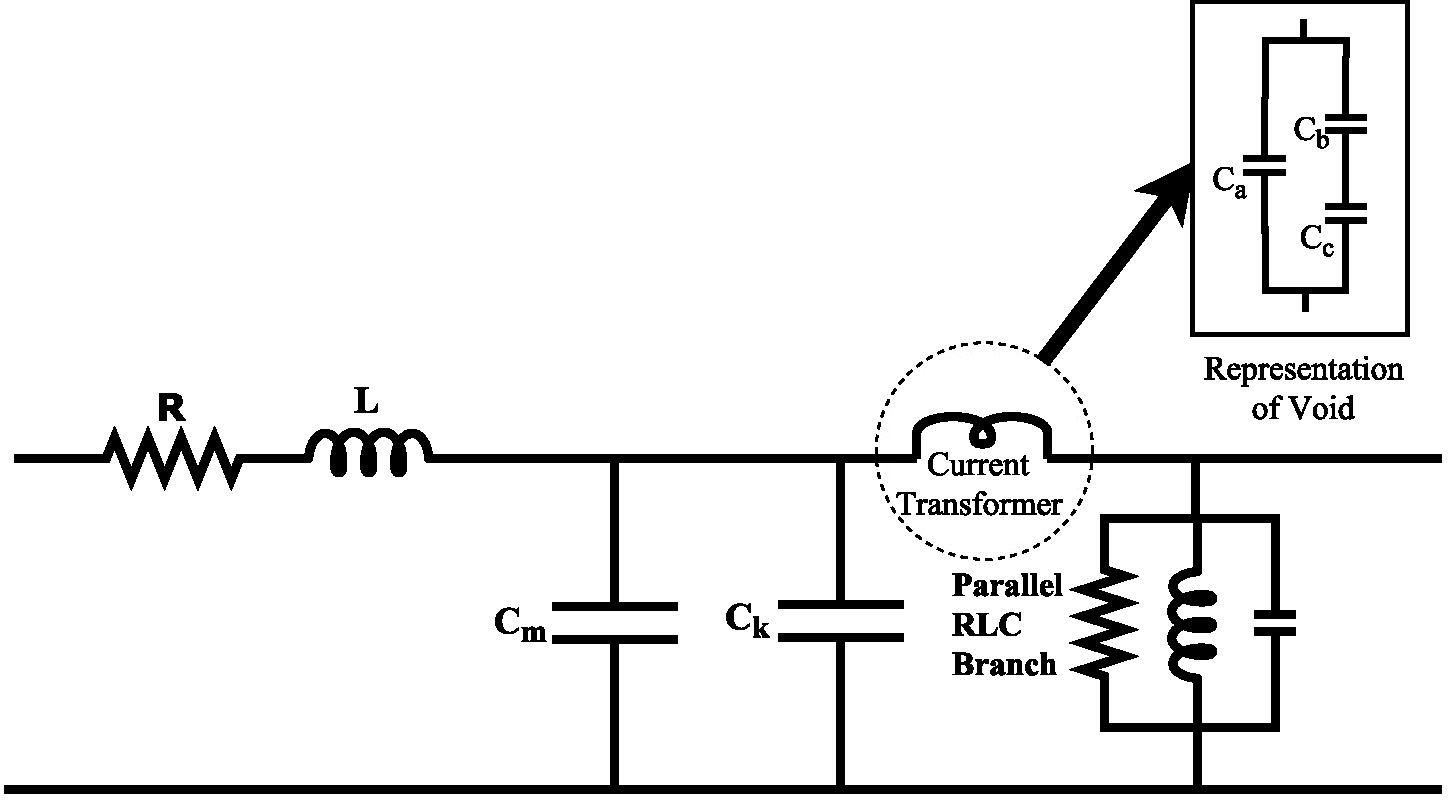
\includegraphics[width=\textwidth]{SimulationModelforHighVoltageCurrentTransformers}
\caption{Simulation Model for High Voltage Current Transformers in Steady State Condition}
\label{fig:Simulation Model for High Voltage Current Transformers in Steady State Condition}
\end{figure}

To study partial discharge pulses due to various sizes of voids capacitor circuit is considered with capacitance $C_b$ and $C_c$ in series and $C_a$ in parallel\setlength{\parskip}{1em}.

The void will represent various capacitance which is named as $C_a$, $C_b$, $C_c$. $C_a$ is the capacitance of discharge free oil insulation of the current transformer. $C_b$ is capacitance in series of void C under consideration. $C_c$ is the capacitance of void.
 
The values of capacitance are $C_a > C_b > C_c$

For the Simulink model to run during steady state conditions, various sizes of voids are considered. The capacitance $C_a$, $C_b$, $C_c$ are calculated for each size of voids. The sample size for the cube for calculation purpose considered as 20x20x6 mm. The detail values of capacitance are shown in the table \ref{table:Values of Capacitance for Different Void Sizes}.

Simulation Model for High Voltage Current Transformers in Steady State Condition derived and concluded, The values of partial discharge depends upon the size of the void, applied voltage and dielectric strength of insulating material From the waveforms generated for the various magnitude of the void, magnitude, number of PDs, Distribution of discharge were studied\setlength{\parskip}{0em}.

\subsection[Simulation model for high voltage current transformers in short circuit and transient condition]{Simulation model for high voltage current\\transformers in short circuit and\\transient condition}

\begin{figure}[h!]
\centering
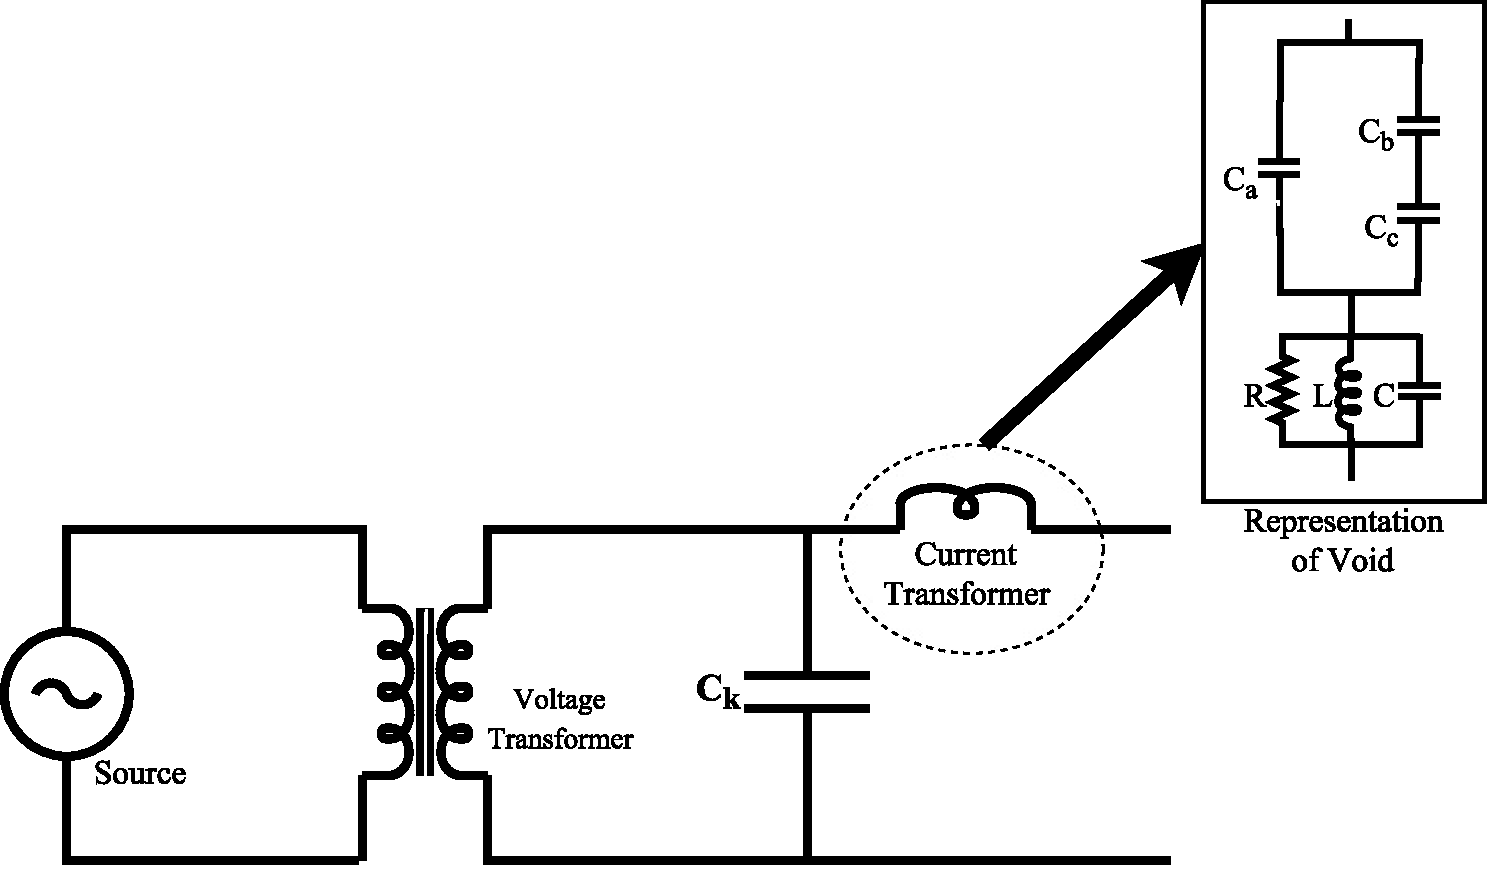
\includegraphics[width=\textwidth]{SimulationModelofPDMeasurementinTransientCondition}
\caption{Simulation Model of PD Measurement in Transient Condition}
\label{fig:Simulation Model of PD Measurement in Transient Condition}
\end{figure}

To Partial discharge process has been initiated for voltage 145 kV and various sizes of voids. Simulink model was run for various void dimensions. Calculated Capacitance values for $C_a$, $C_b$, $C_c$ were given to the circuit. Partial discharge pulses were recorded and studied. With the short circuit and transients, the partial discharge density and magnitudes are very high and thick. The waveforms will show this phenomenon on partial discharge waveforms.

\pagebreak 
\section{Analytical Models}
\subsection[Mathematical model of high voltage current transformers]{Mathematical model of high voltage\\current transformers}
Models for oil filled current transformers with specifications mentioned above are considered for making an analytical model.

\begin{figure}[h!]
\centering
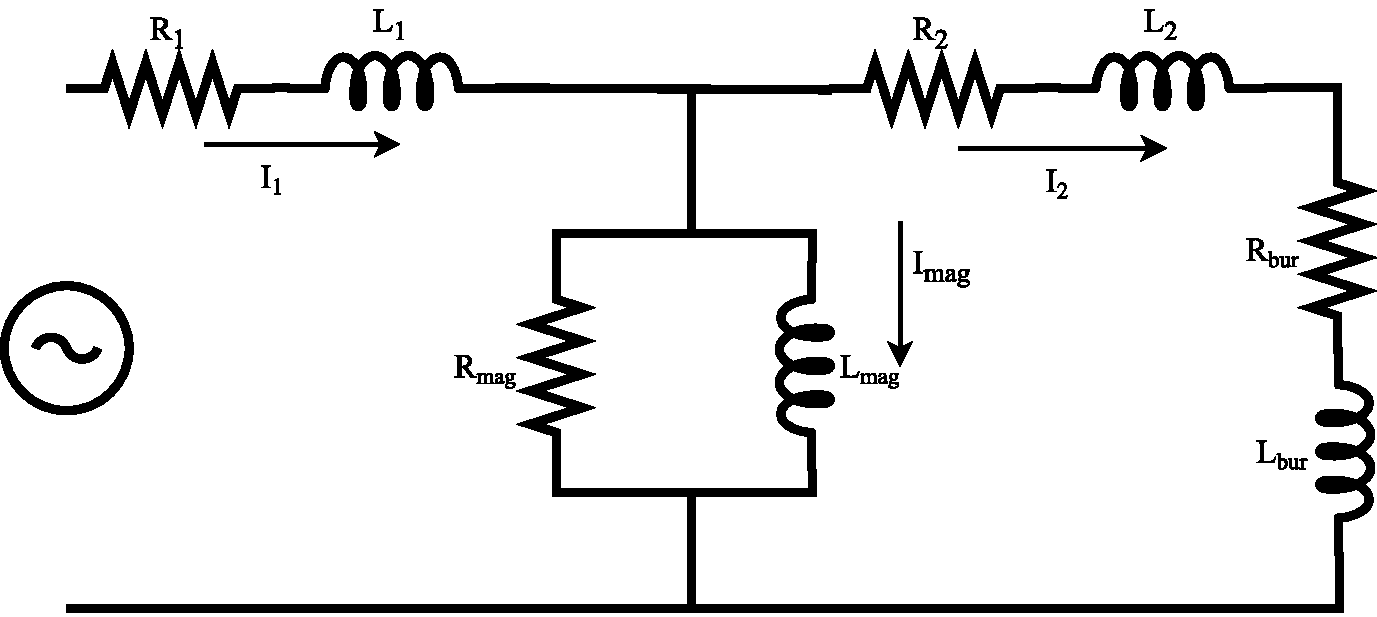
\includegraphics[width=\textwidth]{MathematicalModelofHighVoltageCurrentTransformer}
\caption{Mathematical Model of High Voltage Current Transformer}
\label{fig:Mathematical Model of High Voltage Current Transformer}
\end{figure}

\begin{tabbing}
paragraph \quad 	\= 	paragraph \kill
$R_1 L_1$			\> - Primary leakage impedance \\
$R_2 L_2$ 			\> - Secondary leakage impedance\\
$R_{bur} L_{bur}$	\> - Burden impedance\\
$i_{mag}$			\> - Current derived by the magnetizing branch\\
$i_{fe}$			\> - Current derived by the branch representing core losses.
\end{tabbing}

$i_p - i_{mag}+ i_{sec}$

The flux changes with magnetic current. Writing the equation for current flowing in the magnetizing path with initial data and \textit{w.r.t} time new. The flux will be variable\setlength{\parskip}{1em}.

The mathematical model represents electrical circuit of current transformers with primary and secondary impedances, current in various branches and core loss in the circuit.

$R_1 L_1$ is the resistance and inductance of primary winding, which is 145 kV line and carrying current from 100 A to 3000 A depending upon circuit and acts as the primary of current transformers.

$R_2 L_2$ is resistance and inductance of secondary winding which is carrying a current of 1 A or 5 An in the secondary of current transformers.
 
The magnetizing of cores are represented by a middle link with magnetizing current and electric burden on the system.

This mathematical circuit helps in evaluating the performance of the current transformer in normal working condition and during a short circuit and transient conditions \cite{harrold1985influence}.

With this mathematical representation, any current transformer can be represented in a mathematical model with the values of circuit impedance of the primary and secondary circuit. This will help mathematically to derive the effective performance in the long term\setlength{\parskip}{0em}.  

\subsection{Mathematical model of void in oil insulation}
\subsubsection{Partial discharge equivalent circuit model}
The phenomenon of partial discharge initiates in the voids present in insulating material oil or paper in 145 kV current transformers. The dielectric strength of the insulating material is very high which can sustain electrical stresses inside the instruments. With the presence of a void, the dielectric strength gets reduced, and electric discharge gets initiated. A common source of Partial discharge in solid dielectrics are voids present in the High Voltage Current Transformers. Since voids are the main source of partial discharges, it is necessary to study a mathematical model of partial discharge inside insulation oil or paper. With the period and continuous electrical stresses, insulation deterioration starts and breaks when electrical stress in the void is more than the dielectric strength of the complete insulating material. The size of void plays a major role in discharge phenomenon, and bigger size of voids can lead to complete breakdown of current transformers.\\

For the study purpose, we have considered void in the insulating material oil and paper with specific dimensions. In relation to void dimensions, the capacitance values are calculated. 

\begin{figure}[h!]
\centering
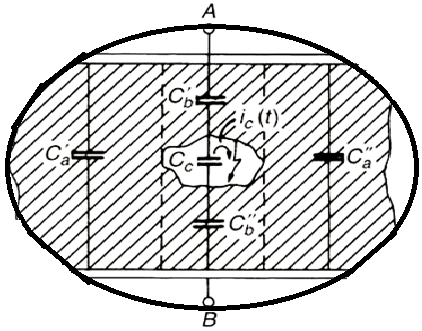
\includegraphics[width=\textwidth]{DielectricMaterialWithaCavity}
\caption{Dielectric Material With a Cavity}
\label{fig:Dielectric Material With a Cavity}
\end{figure}

Figure \ref{fig:Dielectric Material With a Cavity} represents a gas filled void in as capacitor. The partial discharge in void depends on the relative permittivity of the material used and depend on the electrical stress generated. The various capacitance is formed in the geometry sample under consideration.

$C_c$ is the void capacitance\\
$C_b$ is the series capacitance with void\\
$C_a$ is the capacitance of insulation \\
$C_b'$ is capacitance between void and electrode A\\
$C_b''$ is capacitance between void and electrode B\\
Two sides of healthy capacitance are represented by $C_a'$ and $C_a''$. \\
Total capacitance of healthy insulation is $C_a$= Capacitance of both sides of voids, addition of $C_a$ and $C_b$\\
And Similarly, the capacitance in series with void is calculated with capacitance in parallel $C_b = C_b' C_b''/ C_b'+C_b''$.\\
In general $C_a \gg C_b \gg C_c$

\begin{figure}[h!]
\centering
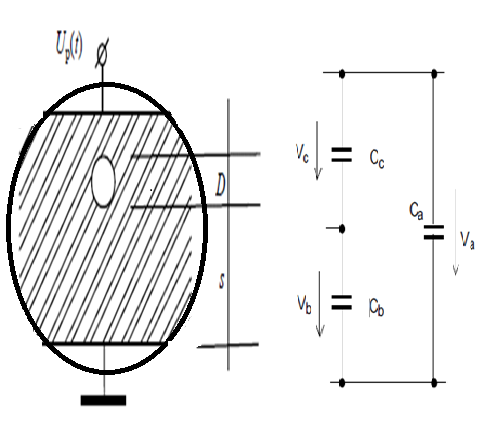
\includegraphics[width=\textwidth]{EquivalentCircuitofaCavityEnclosedinaSolidInsulatingMaterial}
\caption{Equivalent Circuit of a Cavity Enclosed in a Solid Insulating Material}
\label{fig:Equivalent Circuit of a Cavity Enclosed in a Solid Insulating Material}
\end{figure}

The classical model (or abc model or the Gemant- von Philippo model) is given schematically in Fig. 1. The void taken for calculating capacitance is represented as $C_a$ the capacitance of Insulation, $C_b$ as the capacitance of next to void and $C_c$ is the capacitance of void. The voltage across the cavity can be given by 

\begin{equation}
V_c = V_a \frac{C_b}{C_b + C_c}
\end{equation}

The important factor for partial discharge characteristics is void parameters. Partial discharge pulses vary according to the size of the void. Voids can be represented as cylindrical, cubical, rectangular or of irregular shape, \textit{etc}. The capacitance value will change based on the dimensions of voids hence partial discharge, and related parameters will change.

\begin{figure}[h!]
\centering
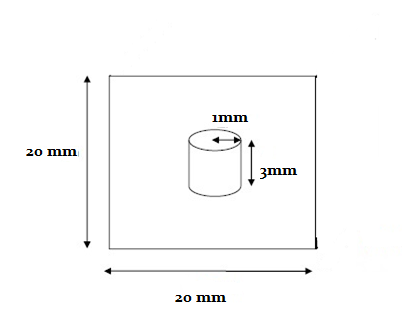
\includegraphics[width=\textwidth]{RepresentationofVoidinOilFilledCurrentTransformer}
\caption{Representation of Void in Oil Filled Current Transformer}
\label{fig:Representation of Void in Oil Filled Current Transformer}
\end{figure}

The object is made up of impregnated paper and represented as three capacitors. Voids are considered in this insulation as per above considerations three capacitance are calculated $C_a$, $C_b$ and $C_c$.

The relative permittivity of Dielectric material considered in this exercise are :

Impregnated Paper Relative permittivity $\varepsilon_r = 5$\\
Free Space Relative permittivity $ \varepsilon_0 = 8.852 \times 10^{-12} F/m$\\
Gap between electrodes $d = 0.005 m$

\subsubsection{Electrical circuit illustrating the partial discharge measurement}
Measurement of Partial Discharge is done to ascertain the healthy condition of current transformers. The test current transformers are connected to the measuring circuit and will measure PD in nano Coulomb. The normal, acceptable limit is up to 10 pC. The impedance of test measuring equipment also has the effect on calculating PD parameters. The circuit diagram shown in figure 4 represents Vs. voltage source, Z impudence of test circuit \cite{harrold1985influence}.

\begin{figure}[h!]
\centering
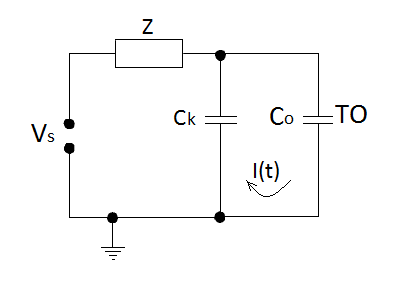
\includegraphics[width=\textwidth]{ElectricalCircuitforPrincipleofPDMeasurement}
\caption{Electrical Circuit for Principle of PD Measurement}
\label{fig:Electrical Circuit for Principle of PD Measurement}
\end{figure}

When the phenomenon of discharge occurs the voltage across test object reduces by $\Delta V$ Capacitance of test CT can be defined as 

\[
C_o \approx C_a + C_b~~~~~~\text{(assuming } C_c \text{ to be negligibly small).} 
\]

If $C_k \gg C_o$ the charge transfer is given by 

\begin{align}
q &= \int i(t) dt \approx (C_a + C_b)\Delta V \\
\text{Now~~} \Delta V &= \frac{C_b}{C_a + C_b} \Delta V_c \\
\Delta V &= \frac{q}{C_a + C_b}\\
i.e. &~~~~\frac{q}{C_a + C_b} = \frac{C_b}{C_a + C_b}  \Delta V_c \\
q &= C_b \Delta V_c
\end{align}

$q$ in above equation is defined as apparent charge and $\Delta V_c$ voltage drop across the cavity in the insulating material

\begin{figure}[h!]
\centering
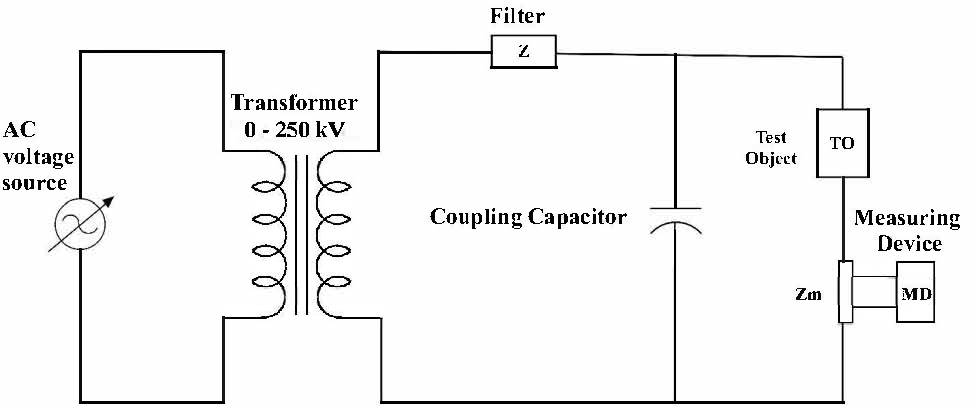
\includegraphics[width=\textwidth]{ConventionalPDmeasurement}
\caption{Conventional PD measurement}
\label{fig:Conventional PD measurement}
\end{figure}

The partial discharge phenomenon initiates the breakdown of dielectric and leads to the formation of the arc which is flow of electrons across the void. The electronics flow faster rate and can be represented in the form of pulses in the waveform. The flow of electronics which has –ve charge generate discharge $i = dq / dt$. During partial discharge phenomenon, also positive ion is created, and disturbances in voids are created. This process is detected by the coupling capacitor in the circuit\setlength{\parskip}{1em}.

Partial discharges in the current transformers depend upon capacitance values of voids and insulating material.
 
In this experiments, various sizes of voids are considered such as cylindrical, rectangular, square, ellipse with various dimensions. The cube sample considered is $20 \times 20 \times 6$

The capacitance $C_a$, $C_b$, $C_c$ are formed in sample size are considered, and values of capacitance are calculated with the formulas : 

\begin{align}
C_c &= \frac{\varepsilon_0 \times r^2 \times \pi}{h}\\
C_b &= \frac{\varepsilon_0 \times \varepsilon_r \times r^2 \times \pi}{d - h}\\
C_a &= \frac{\varepsilon_0 \times \varepsilon_r \times (A - r^2 \pi)}{d}
\end{align}

The voltage applied to current transformer test object 145 kV and 50 Hz frequency. To study capacitance values are calculated in the form of $C_a$, $C_b$, $C_c$. enclosed shows all calculated values. 

In the circuit used for calculating partial discharges, the Test instrument is considered, and components values are considered in simulation circuit.

\begin{tabular}{l  l}
1. High Voltage Transformer		&: Primary 230 V; Secondary 145 kV\\
2. Value of Measuring Capacitor	& : 400/1600 pF\\
3. Value of Coupling Capacitor	& : 1000 $\mu$F\\
\textbf{RLC values of Detector circuit} & {}\\
4. Resistance					& : 500 $\Omega$\\
5. Inductance	 				& : 0.065 mH\\
6. Capacitance 	 				& : 0.47 $\mu$F
\end{tabular}

Simulation has been done for high voltage current transformers to evaluate the performance during Steady State Condition and Short Circuit and Transient conditions. The performance has been evaluated by considering various voids and calculating the capacitance $C_a$, $C_b$, $C_c$. With this values put in Simulation model, the performance in the form of the waveform can be generated in Matlab\setlength{\parskip}{0em}.

\section[Manufacturing Processes and Actions to Avoid Partial Discharge]{Manufacturing Processes and Actions to\\Avoid Partial Discharge}
Partial Discharge measured in Current Transformer acceptable limit is between 5 pC to 10 pC Out of the results measured segregated CT where Partial Discharge is more than 10 pC After the Analysis, following reasons observed which lead to higher PD

\begin{enumerate}
\item High Vacuum Level
\item low Temperature
\item High Oil Flow Rate
\end{enumerate}

During manufacturing process the parameters specified are :

Vacuum Level $5 \times 10^{-4} = 0.5 mbar$\\
Temperature 138\textdegree C \\

Oil flow rate Initial for 6 hrs 0.5 lit/hr\\
Middle for 8 hrs 4 lit/hr\\
Final for 8 Hrs 14 lit/hr\\
Analysis of Partial Discharge in Current Transformers\\
a) Low vacuum level less then 0.5 mbar\\
Low vacuum extracts less moisture.\\
Retained moisture leads to Partial Discharge.\\
Evacuation system is designed for high vacuum and low temp.\\
If vacuum is high, then evaporation rate is less then100\textdegree C\\
Dielectric strength of impregnated insulation should be more, if not voids will be formed \\
b) Low temp of oil less then138\textdegree C\\
If the temperature of the oil is less then138\textdegree C, moisture contents in the insulation will not be removed and can form voids in the insulating material.

The insulation paper layers are around 22 nos, the temp must reach the inner most layer and remove the moisture contents.

The Nonremoval of moisture of insulating material will reduce the insulating strength and can discharge with high magnitude pulses.

c) Effect of High Oil flow rate
During the filling of transformer oil in current transformer care should be taken to control flow rate otherwise chances of forming bubbles in oil and air may trap inside. 

Hence oil flow should be slow to the extent paper absorbs oil. If it is more paper will not absorb oil completely and simultaneously air bubble formation in the oil tank.

The elasticity of paper that provides compression pressure on the inner layer will not allow the air to trap. The paper used in the sequence of Non stretched, Light Stretched and crepe paper.

The quality of insulation paper should match the absorption with the rate of oil filled in current transformers. If the absorption rates are not matched, there will be chances of forming voids and Voids are the potential for partial discharge.

\subsection{Service experience analysis}

\subsubsection{Case 1}
Current Transformer, 145 kV oil, filled after 15 years working in substation due to the explosion of the bushing. This failure has resulted in damage to secondary winding insulation, contamination of the toroidal cores and shell assembly, rupture of porcelain and contamination of the oil.
 
This case is the total breakdown of insulation dielectric strength and the result of persistent partial discharge at some area in oil, paper, copper, bushing, core or another part. 

\subsubsection{Case 2}
The on line current transformer after long service was taken for partial discharge measurement and taken for life assessment. 

The oil insulation must have undergone various transient conditions during long term operation. The deterioration of insulation strength can be evaluated from a breakdown voltage and measurement of Tan delta.

BDV of oil 90 kV\\
Tan delta 0.00019\\

The Service condition has shown good results of the insulation strength of oil.\\
The current transformer oil contains the following chemicals:\\

\begin{tabular}{| l l | l l | l l | l l | }
\hline
$H_2$ & :0.034 & $CH_4$ & :0.52 & $C_2H_2$ & :0.162 &  $C_2H_4$ & :0.21\\ \hline
$C_2H_6$ & :0.60 & $CO$ & :0.067 & $CO_2$& :0.12 & $N_2$ & :4.7 \\ \hline 
\end{tabular}

\subsection{Specifications of current transformers}
Current Transformer 1
\begin{table}[h!]
\caption{Specification of Current Transformer 1}
\label{table:Specification of Current Transformer 1}
\centering
\begin{tabular}{|l|c|}
\hline 
CT Ratio &  3000/1  \\ \hline 
Core Size & $225 \times 275 \times 50$ \\ \hline 
No. of turns on Secondary  & 3000 \\ \hline 
Burdon & 30 VA  \\ \hline 
KPV (V)  & 20 mA @vk/2 \\ \hline 
Resistance  & 12 $\Omega$\\ \hline 
Excitation current & 12 mA \\ \hline 
ISF  & 5 \\ \hline 
Accuracy Class  & 0.5 \\ \hline 
\end{tabular} 
\end{table}

\clearpage
Current Transformer 2
\begin{table}[h!]
\caption{Specification of Current Transformer 2}
\label{table:Specification of Current Transformer 2}
\centering
\begin{tabular}{|l|c|}
\hline 
CT Ratio &  2400/1  \\ \hline 
Core Size & $220 \times 400 \times 45$ \\ \hline 
No. of turns on Secondary  & 2400 \\ \hline 
Burdon & No burdon  \\ \hline 
I excitation   & 100 vk \\ \hline 
Resistance  & 18 $\Omega$ \\ \hline 
Excitation current & 28 mA \\ \hline 
ISF  & 5 \\ \hline 
Accuracy Class  & PS \\ \hline 
\end{tabular} 
\end{table}

Current Transformer 3
\begin{table}[h!]
\caption{Specification of Current Transformer 3}
\label{table:Specification of Current Transformer 3}
\centering
\begin{tabular}{|l|c|}
\hline 
CT Ratio &  200/1  \\ \hline 
Core Size & $220 \times 405 \times 40$ \\ \hline 
No. of turns on Secondary  & 200 \\ \hline 
Burdon & No burdon  \\ \hline 
KPV (V)   & 20 mA vk/2 \\ \hline 
Resistance  & 11 $\Omega$\\ \hline 
Excitation current & 12 mA \\ \hline 
ISF  & 5 \\ \hline 
Accuracy Class  & 0.2 S \\ \hline 
\end{tabular} 
\end{table}

\clearpage
Current Transformer 4
\begin{table}[th!]
\caption{Specification of Current Transformer 4}
\label{table:Specification of Current Transformer 4}
\centering
\begin{tabular}{|l|c|}
\hline 
CT Ratio &  600/1  \\ \hline 
Core Size & $215 \times 300 \times 25$ \\ \hline 
No. of turns on Secondary  & 150 \\ \hline 
Burdon & No burdon  \\ \hline 
I excitation   & 100 vk \\ \hline 
Resistance  & 0.2 $\Omega$ \\ \hline 
Excitation current & 340 mA \\ \hline 
ISF  & 5 \\ \hline 
Accuracy Class  & 5P \\ \hline 
\end{tabular} 
\end{table}

\newgeometry{left=1.5in,right=1in,top=0.8in,bottom=1in}
\begin{table}[h!]
\caption{Results of Accuracy testing of Current Transformers in Steady State and transients}
\label{table:Results of Accuracy testing of Current Transformers in Steady State and transients}
\renewcommand{\arraystretch}{1.3}
\centering
\begin{tabular}{|>{\centering\arraybackslash}m{0.6in}|>{\centering\arraybackslash}m{0.5in}|>{\centering\arraybackslash}m{0.6in}|>{\centering\arraybackslash}m{0.8in}|>{\centering\arraybackslash}m{0.7in}|>{\centering\arraybackslash}m{0.8in}|>{\centering\arraybackslash}m{0.7in}|}
\hline 
\multicolumn{3}{|c|}{} & \multicolumn{2}{c|}{Steady state} & \multicolumn{2}{c|}{Transients} \\ \hline 
Ratio & Burden  & Primary Current & Ratio Error  & Phase Error  & Ratio Error  & Phase Error  \\
(Amp/) & (VA) & (\%) & (\%) & minutes & (\%) & minutes \\ \hline \hline
\multirow{8}{*}{3000/1} & \multirow{4}{*}{30} & 120 & 0.342 & 0.56 & 2.345 & 3.423 \\ \cline{3-7}
 &  & 100	& 0.331 & 0.67 & 2.456 & 3.674\\ \cline{3-7}
 &  & 20  & 0.129 & 2.56 & 1.341 & 2.874 \\ \cline{3-7}
 &  & 5   & 0.012 & 3.98 & 1.456 & 2.712\\ \cline{2-7}
 & \multirow{4}{*}{7.5} & 120&0.256 & 0.35 & 2.023 & 4.512 \\ \cline{3-7}
 & & 100&0.237 & 0.45 & 2.402 & 4.521 \\ \cline{3-7}
 & & 20 & 0.148 & 0.56 & 1.890 & 2.98 \\ \cline{3-7}
 & & 5& 0.126 & 0.21 & 1.562 & 2.453 \\ \hline \hline
2400/1 & 0 & 100 & -0.034 & 0.96 & 5.670 & 15.59 \\ \hline \hline
600/5 & 10 & 100 & 0.007 & 0.29 & 3.15 & 9.23 \\ \hline \hline
\multirow{8}{*}{200/1} &\multirow{4}{*}{30} & 120 & 0.116 & 0.33 & 1.568 & 1.89 \\ \cline{3-7}
& & 100 & 0.112 & 0.34 & 1.558 & 1.87\\ \cline{3-7}
& & 20 & 0.076 & 1.78 & 2.321 & 4.56\\ \cline{3-7}
& & 5 & 0.053 & 3.47 & 2.291 & 9.37 \\ \cline{2-7}
& \multirow{4}{*}{7.5} & 120 & 0.158 & 0.18 & 1.628 & 1.75\\ \cline{3-7}
& & 100 & 0.157 & 0.21 & 1.601 & 1.71 \\ \cline{3-7}
& & 20 & 0.153 & 0.4 & 1.289 & 2.36\\ \cline{3-7}
& & 5 & 0.144 & 0.14 & 1.243 & 2.59 \\ \hline 
\end{tabular} 
\end{table}
\restoregeometry

Readings of Ratio error and phase error took for different CT ratios and accuracy class. The performance in the steady state shows accuracy results as per IS/IEC standards. After transient conditions readings and thus performance of current transformers abruptly changes, the accuracy results are not in the acceptable limit as per IS/IEC standard.

The Capacitance values were calculated for different shapes rectangle, square, circle, ellipse and variable sizes in height and radius. The capacitance $C_a$, $C_b$, $C_c$ were calculated for different sizes. These values of capacitance were utilized in Simulink model for waveforms in steady state and transient conditions.

\newgeometry{left=1in,right=1in,top=0.5in,bottom=1in}
\begin{table}[h!]
\caption{Values of Capacitance for Different Void Sizes}
\label{table:Values of Capacitance for Different Void Sizes}
\centering
\small
\begin{tabular}{|c|c|c|c|c|c|c|}
\hline 
Void & \multicolumn{2}{c|}{Void} & Dimensions & \multicolumn{3}{c|}{Capacitance}  \\ 
\hline 
Geometry & Height & Radius & • &  All Insulation & Series with Void & Void \\ 
• & m & m & m & $C_a F$ & $C_b F$ & $C_c F$ \\ \hline \hline 
			& 0.005 & 0.001 & .020$\times$.020$\times$.006  & 4.1943$e^{-13}$ & 1.39021$e^{-13}$ & 5.56083$e^{-15}$ \\ \cline{2-7}
Rectangle	& 0.005 & 0.002	& 								& 3.4992$e^{-13}$ & 5.56083$e^{-13}$ & 2.22433$e^{-14}$\\ \cline{2-7}
y-Axis		&0.005 & 0.003	&								& 2.34069$e^{-13}$ & 1.25119$e^{-12}$ & 5.00474$e^{-14}$ \\ \cline{2-7}
 			&0.005 & 0.004 	&								& 7.18782$e^{-14}$ & 2.22433$e^{-12}$ & 8.89732$e^{-14}$ \\ \cline{2-7}
 			&0.005 & 0.005 	& 								& 1.36653$e^{-13}$ & 3.47552$e^{E-12}$ & 1.39021$e^{-13}$ \\ \hline \hline		
\multirow{4}{*}{Square}&0.001 & 0.001& .020$\times$.020$\times$.006& 4.1943$e^{-13}$  & 2.78041$e^{-14}$ & 2.78041$e^{-14}$ \\ \cline{2-7}
 			&0.002&0.002	& 								& 3.4992$e^{-13}$  & 1.39021$e^{-13}$ &1.11217$e^{-13}$ \\ \cline{2-7}
 			&0.003&0.003	& 								& 2.34069$e^{-13}$ & 4.17062$e^{-13}$ &2.50237$e^{-13}$ \\ \cline{2-7}
 			&0.004&0.004	& 								& 7.18782$e^{-14}$ & 1.11217$e^{-12}$ &4.44866$e^{-13}$ \\ \hline \hline
			&0.001&0.005	&.020$\times$.020$\times$.006	& 1.36653$e^{-13}$ & 6.95103$e^{-13}$ &6.95103$e^{-13}$ \\ \cline{2-7}
Rectangle	&0.002&0.005	& 								& 1.36653$e^{-13}$ & 8.68879$e^{-13}$ &3.47552$e^{-13}$ \\ \cline{2-7}
x-Axis		&0.003&0.005	& 								&1.36653$e^{-13}$  &1.15851$e^{-12}$  &2.31701$e^{-13}$ \\ \cline{2-7}
 			&0.004&0.005	& 								&1.36653$e^{-13}$  &1.73776$e^{-12}$  &1.73776$e^{-13}$ \\ \cline{2-7}
 			&0.005&0.005	& 								&1.36653$e^{-13}$  &3.47552$e^{-12}$  &1.39021$e^{-13}$ \\ \hline \hline
\multirow{7}{*}{Ellipse}&0.001&0.002&.020$\times$.020$\times$.006&3.4992$e^{-13}$   &1.11217$e^{-13}$  &1.11217$e^{-13}$ \\ \cline{2-7}
 			&0.001&0.003	& 								&2.34069$e^{-13}$  &2.50237$e^{-13}$  &2.50237$e^{-3}$ \\ \cline{2-7}
 			&0.001&0.004	& 								&7.18782$e^{-14}$  &4.44866$e^{-13}$  &4.44866$e^{-13}$ \\ \cline{2-7}
			&0.002&0.005&									&1.36653$e^{-13}$&8.68879$e^{-13}$&3.47552$e^{-13}$ \\ \cline{2-7}
 			 &0.003&0.004	& 									&7.18782$e^{-14}$&7.41444$e^{-13}$&1.48289$e^{-13}$ \\ \cline{2-7}
 			 &0.003&0.005	& 									&1.36653$e^{-13}$&1.15851$e^{-12}$&2.31701$e^{-13}$ \\ \cline{2-7}
 			&0.004&0.005	& 									&1.36653$e^{-13}$&1.73776$e^{-12}$&1.73776$e^{-13}$ \\ \hline \hline
\multirow{4}{*}{Medium Voids}&0.01&0.015		&.020$\times$.020$\times$.006		&3.47109$e^{-10}$&7.81991$e^{-12}$&2.78041$e^{-13}$\\ \cline{2-7}
 			&0.009&0.012	& 									&2.77599$e^{-10}$&6.67299$e^{-12}$&2.50237$e^{-13}$ \\ \cline{2-7}
 			&0.008&0.01		& 									&2.31259$e^{-10}$&6.95103$e^{-12}$&2.22433$e^{-13}$ \\ \cline{2-7}
 			&0.007&0.008	& 									&1.84918$e^{-10}$&6.67299$e^{-12}$&2.50237$e^{-13}$ \\ \hline \hline
\multirow{3}{*}{Big Voids}&0.5&0.3	&.020$\times$.020$\times$.006&6.95059$e^{-9}$&2.53277$e^{-11}$&1.39021$e^{-11}$ \\ \cline{2-7}
 			&0.7&0.4		& 									&9.2676$e^{-9}$&3.20509$e^{-11}$&1.94629$e^{-11}$ \\ \cline{2-7}
 			&0.9&0.5		& 									&1.39016$e^{-8}$&5.59815$e^{-11}$&2.50237$e^{-11}$ \\ \hline
\end{tabular} 
\end{table}
\clearpage

\newgeometry{left=1in,right=1in,top=1in,bottom=1in}
\begin{table}[h!]
\caption{Values of Capacitance For Big Void Sizes}
\label{table:Values of Capacitance For Big Void Sizes}
\centering
\begin{tabular}{|c|c|c|c|c|c|c|}
\hline 
Void & \multicolumn{2}{c|}{Void} & Dimensions & \multicolumn{3}{c|}{Capacitance}  \\ 
\hline 
Geometry & Height & Radius & • &  All Insulation & Series with Void & Void \\  
• & m & m & m & $C_a F$ & $C_b F$ & $C_c F$ \\ \hline \hline
\multirow{6}{*}{Big Voids}&0.1	&0.3&.020$\times$.020$\times$.006	&2.52503$e^{-13}$	&1.33105$e^{-14}$	&2.50237$e^{-13}$\\ \cline{2-7}
		 &0.2	&0.3& 								&2.52503$e^{-13}$	&6.44941$e^{-15}$	&1.25119$e^{-13}$\\ \cline{2-7}
 		 &0.3	&0.3&								&2.52503$e^{-13}$	&4.25573$e^{-15}$	&8.34124$e^{-14}$\\ \cline{2-7}
 		 &0.4	&0.3& 								&2.52503$e^{-13}$	&3.1756$e^{-15}$	&6.25593$e^{-14}$\\ \cline{2-7}
 		 &0.5	&0.3& 								&2.52503$e^{-13}$	&2.53277$e^{-15}$	&5.00474$e^{-14}$\\ \cline{2-7}
 		 &0.6	&0.3& 								&2.52503$e^{-13}$	&2.10637$e^{-15}$	&4.17062$e^{-14}$\\ \hline
\end{tabular} 
\end{table}


\begin{table}[h!]
\caption{Values of Capacitance For Irregular Shape}
\label{table:Values of Capacitance For Irregular Shape}
\centering
\begin{tabular}{|c|c|c|c|c|c|c|}
\hline 
Void & \multicolumn{3}{c|}{Void Dimensions} & \multicolumn{3}{c|}{Capacitance}  \\ 
\hline 
Geometry & Height & Radius & Area &  All Insulation & Series with Void & Void \\  
• & m & m & m\textsuperscript{2} & $C_a F$ & $C_b F$ & $C_c F$ \\ \hline \hline
\multirow{5}{*}{Irregular Shape}&0.005	&0.001	&0.0000032	&4.19$e^{-13}$	&1.39$e^{-13}$	&2.39$e^{-12}$ \\ \cline{2-7}
				&0.005	&0.002	&0.0000039	&3.50$e^{-13}$	&5.56$e^{-13}$	&9.62$e^{-12}$ \\ \cline{2-7}
 				&0.005	&0.003	&0.0000045	&2.34$e^{-13}$	&1.25$e^{-12}$	&2.17$e^{-11}$ \\ \cline{2-7}
 				&0.005	&0.004	&0.0000055	&7.19$e^{-14}$	&2.22$e^{-12}$	&3.86$e^{-11}$ \\ \cline{2-7}
 				&0.005	&0.005	&0.0000032	&1.37$e^{-13}$	&3.48$e^{-12}$	&6.03$e^{-11}$ \\ \hline
\end{tabular} 
\end{table}

The capacitance values for different void sizes $C_a$, $C_b$, $C_c$ are calculated and tabulated. These capacitance values are used in Simulink model for waveform studies. The capacitance values decrease with increase in void dimensions.

The capacitance values $C_a$, $C_b$, $C_c$ calculated above for different void sizes are used in Simulink model, and waveform pulses are studied for the effect in steady state and transient conditions. 

\restoregeometry